\chapter{Planificación e seguimento}
\minitoc
% \label{chap:Planificacioneseguimento}
% \vspace{0.5cm}

%%%%%%%%%%%%%%%%%%%%%%%%%%%%%%%%%%%%%%%%%%%%%%%%%%%%%%%%%%%%%%%%%%%%%%%%%%%%%%%%
% Objetivo:                        %
%%%%%%%%%%%%%%%%%%%%%%%%%%%%%%%%%%%%%%%%%%%%%%%%%%%%%%%%%%%%%%%%%%%%%%%%%%%%%%%%

  \lettrine{N}{este} capítulo detallaremos a planificación e o seguimento 
do proxecto, un proxecto que por diversas circunstancias se dividíu 
principalmente en tres grandes etapas, as dúas primeiras mentres VACmatch era 
unha iniciativa emprendedora baseada nun proxecto software libre e a última 
durante a cal se comezou unha conversión da iniciativa cara un proxecto 
comunitario.

  Durante o desenvolvemento xuridiron tamén diversos acontecementos 
relacionados co proxecto e que tamén é importante resaltar debido a súa 
influencia no desenvolvemento.

  \begin{description}
    \item [Agosto 2015 - Outubro 2015] VACmatch. Validación de negocio.
    \item [Outubro 2015 - Xaneiro 2016] VACmatch. Desenvolvemento de produto.
    \item [Xaneiro 2016 - Xuño 2016] De empresa a comunidade.
  \end{description}


  \section{Validación de negocio (Xullo 2015 -- Novembro 2015)}
  A duración de esta etapa é de aproximadamente 4 meses e ven determinada polos 
primeiros pasos de VACmatch como iniciativa empresarial e que levan a orientar 
o desenvolvemento do produto cara o cliente, comezando con unha serie de 
prototipos para coñecer as suas necesidades e validar a idea de 
negocio.

  Durante o primeiro mes planifícase a realización dun prototipo visual co 
fin de comprobar a usabilidade e consolidar os requisitos dos clientes.
  De seguido, plantéxase crear un pequeno prototipo funcional, un MVP (Mínimo 
Producto Viable) na metodoloxía Lean Startup, co obxectivo de testear as 
necesidades dos clientes e definir o produto final a desenvolver.

    \subsection{Prototipo visual}

      \subsubsection{Planificación e definición da iteración}
      Esta iteración dura un total de 4 semanas de desenvolvemento entre o 15 
de Xullo e o 16 de Agosto e realizase unha visita semanal ao cliente para obter 
feedback e mostrarlle a evolución do prototipo.

      Durante este periodo de un mes de duración planificouse o desenvolvemento 
de unha aplicación moi sinxela e sen funcionalidade, que únicamente permitise 
analizar a usabilidade do sistema e comprobar si é factible adaptar o proceso 
de creación de un acta deportiva, a unha aplicación móbil.

    Así mesmo, ao longo do período realizaranse ata tres visitas a federación 
coa que se traballou dende o primeiro momento para comprobar a experiencia de 
un futuro usuario real da aplicación e obter feedback para futuras melloras.

      \subsubsection{Revisión e feedback}
      Durante as visitas as federacións obtivéronse diversas prospostas que 
levaron a adaptar o prototipo:

      \begin{itemize}
        \item Facer interactiva a aplicación e non mostrar grandes táboas con 
datos.
        \item Todas as accións deben xirar ao redor da acta.
        \item Crear partidos cando non hai cobertura.
      \end{itemize}

      \subsubsection{Tarefas e seguimento}

      A descomposición das tarefas desta iteración son as seguintes:

      \begin{itemize}
        \item Crear esqueleto da aplicación.
        \item Como árbitro quero poder consultar as próximas actas a 
cubrir.
        \item Como árbitro quero poder consultar as actas xa cubertas.
        \item Como árbitro quero poder editar un acta.
        \item Como árbitro quero poder ver un acta.
        \item Como árbitro quero poder ver os xogadores de ambos equipos.
        \item Como árbitro quero poder engadir un evento.
        \item Como árbitro quero poder rematar ou suspender un partido.
        \item Como árbitro quero poder logearme.
        \item Como árbitro quero poder seleccionar cales xogadores de cada 
equipo se atopan no encontro.
        \item Como árbitro quero poder borrar un evento.
        \item Estudio sobre React e Flux.
       \end{itemize}

    \subsection{MVP funcional}

      \subsubsection{Planificación e definición da iteración}
      Esta iteración dura un total de 3 meses e desenvólvese entre o 16 de 
Agosto e o 15 de Novembro, realizando múltiples visitas a federacións e 
asociacións deportivas.

      Unha vez finalizadas as probas visuais e de usabilidade procédese 
a planificar o desenvolvemento para adaptar o prototipo e engadirlle 
funcionalidade sinxela, sen validacións e sen funcionalidade offline, co 
obxectivo de obter un prototipo funcional que poida ser utilizado por usuarios 
reais nun entorno controlado.

      Engadirase funcionalidade para as vistas creadas na iteración anterior, 
comezando polo listado de actas pendentes e rematadas e diversos compoñentes 
xenéricos como os que se utilizan para listar xogadores e outros elementos como 
poden ser as actas.

      Únicamente se engadirá a funcionalidade básica imprescindible para 
xestionar un encontro, excluindo requisitos como a sinatura de actas ou a 
creación offline das mesmas co fin de axilizar as primeiras probas.

      Durante a iteración tamén se farán visitas a federación para mostrar o 
estado do desenvolvemento e para buscar que tamén árbitros reais vexan os 
progresos e proporcionen feedback.

      Unha vez rematada a iteración realizarase o torneo onde probar o 
prototipo desenvolto nun caso real; pódese ver o desenvolvemento de dita 
competición na Sección~\ref{sec:torneo_vacmatch}.

      \subsubsection{Revisión e feedback}
      Durante as visitas as federacións obtivéronse múltiples propostas e 
melloras, moitas das cales será incorporadas ao backlog do proxecto mentres que 
outras serán rexeitadas polo momento ao non considerarse prioritarias ou por 
ser casos de usos moi concretos para esa federación e dificilmente 
extrapolables a outras.

      \textbf{Listaxe de tarefas engadidas ao backlog}.
        \begin{itemize}
          \item Meter xogadores manualmente xa que poden non terse creado no 
sistema de xestión.
          \item Poder ver os eventos de forma sinxela dende a vista de fin de 
partido para que os equipos vexan o que están firmando.
         \item Editar dorsal dos xogadores xa que poden cambiar.
         \item Ter opción de non poñer motivo para as tarxetas.
         \item Mostrar foto de xogador ao engadir un evento.
        \end{itemize}

      \textbf{Listaxe de tarefas rexeitadas polo momento}.
        \begin{itemize}
         \item Ao marcar doble amarela, avisar da expulsión. Moi concreta para 
un deporte, non se implementa de momento.
         \item Mostrar confirmación de que se engadíu un evento.
         \item Avisar aos delegados/personal do clube cando se sube un acta.
         \item Posibilidade de que o árbitro engada un anexo na casa á acta en 
lugar de escribir as incidencias.
        \end{itemize}

      \subsubsection{Tarefas e seguimento}

      As tarefas que se realizarán durante esta iteración son as seguintes:

        \begin{description}
        \item [MVP1] Como árbitro quero poder cargar a lista de actas pendentes.
        \item [MVP2] Como árbitro quero poder cargar a lista de actas rematadas.
        \item [MVP3]Como árbitro quero poder ver os datos dun partido.
        \item [MVP4]Como árbitro quero poder ver a lista de xogadores dun 
equipo.
        \item [MVP5] Como árbitro quero poder seleccionar os xogadores 
presentes no partido.
        \item [MVP6] Como árbitro quero poder engadir un gol a un xogador.
        \item [MVP7] Como árbitro quero poder engadir unha falta a un xogador.
        \item [MVP8] Como árbitro quero poder engadir unha tarxeta (amarela ou 
vermella) a un xogador.
        \item [MVP9] Como árbitro quero poder ver a lista de eventos de un 
partido.
        \item [MVP10] Como árbitro quero poder borrar eventos de un partido.
        \item [MVP11] Como árbitro quero poder engadir incidencias a un partido.
       \end{description}

      Planificouse un total de 65 horas para desenvolver esta iteración que non 
resultaron suficientes, obrigando a facer un total de 10,5 horas extra motivado 
polo descoñecemento da tecnoloxía, formación na que foi preciso invertir un 
maior número de horas das esperadas.

    \subsubsection{I Torneo VACmatch}
    \label{sec:torneo_vacmatch}
    Durante este periodo tamén se planificou a organización dun torneo de 
  fútbol sala a finais do mes de Outubro coa idea de probar en nun entorno real 
  e controlado, os primeiros prototipos desenvoltos.

  Finalmente participaron 6 equipos e mais de 50 persoas durante os dóus días 
que durou o evento, obtendo todo tipo de suxerencias e detectando múltiples 
erros que serán analizados e comentados na seguinte iteración.

  \begin{figure}[h!]
        \begin{center}
        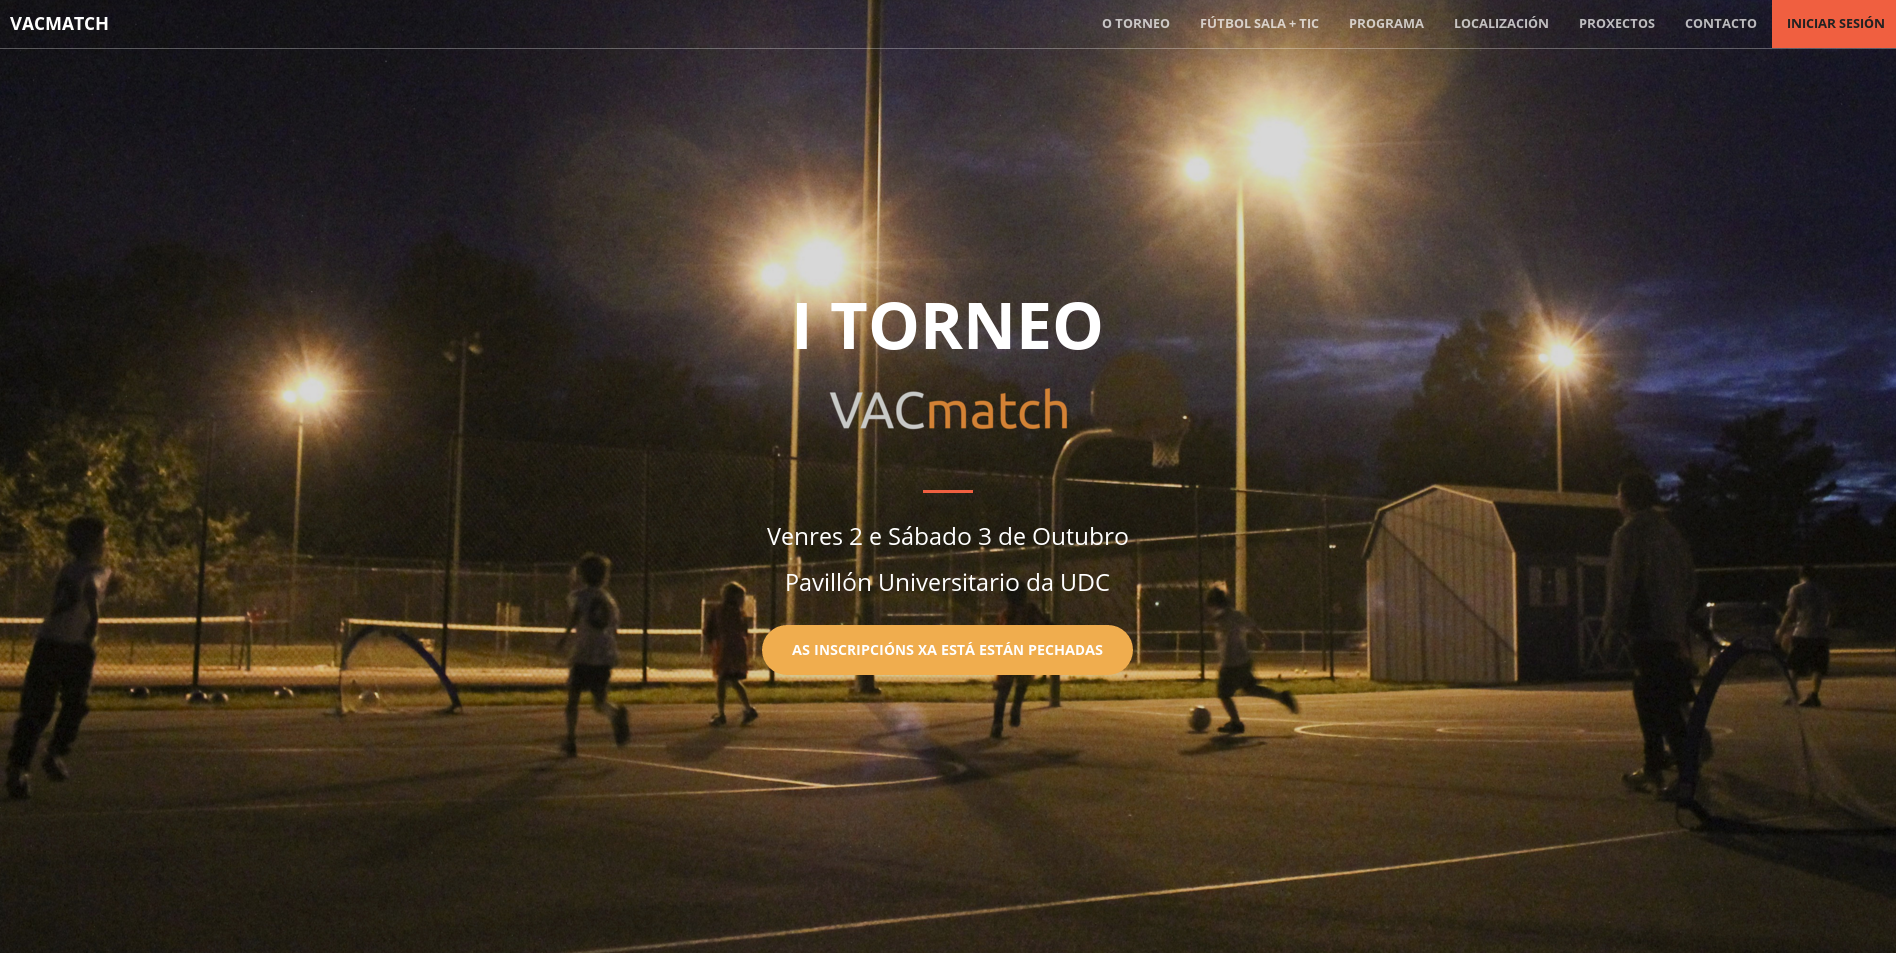
\includegraphics[width=\textwidth]{./img/torneo_vacmatch.png}
        \caption{Web do I Torneo VACmatch}
        \end{center}
  \end{figure}


  \section{Desenvolvemento de produto (Novembro 2015 -- Xaneiro 2016)}
  Tras analizar os problemas e os erros cometidos durante a realización do I 
Torneo VACmatch, e concretamente no funcionamento 
da aplicación móbil durante o 
mesmo, decidíuse comezar novamente dende o principio un proxecto novo en lugar 
de facer unha refactorización do prototipo.

    Durante este tempo decidimos inscribir o proxecto no ``Concurso 
Universitario de Software Libre'' o que incentivou a comezar a escribir un 
blog técnico, a través da conta de Medium\footnote{Medium é unha rede social 
que permite crear e seguir blogs de múltiples temáticas} de VACmatch, no que 
contar os avances que suceden durante o desenvolvemento do proxecto.

  En este periodo de 3 meses de duración planifícase dedicar unha media de 4 
horas diarias a VACmatch Mobile debido a que en paralelo se está a traballar na 
versión de VACmatch Web.

  Así mesmo descontando os múltiples días festivos calculase un total de 208 
horas de traballo divididas en 5 iteracións.

    \subsection{1ª e 2º iteración. Creación do proxecto e xestión de actas}

      \subsubsection{Planificación e definición da iteración}
      Estas iteracións transcorren ao longo do mes de Novembro, adicando 15 
dias a cada unha.

      A primeira céntrase en comezar o desenvolvemento da 
aplicación pensando dende o primeiro momento no funcionamento tanto online 
como offline e controlando os posibles conflictos que poidan suceder entre os 
datos.

      Comézase co estudo da tecnoloxía en profundidade xa que os 
prototipos non utilizaban nin Reflux nin PouchDB e simplemente enviaban os 
datos a unha API remota.

      Créase tamén o proxecto base engadindo a licencia e defínese o modelo de 
datos, que vai cambiar bastante do modelo inicial, pensando para unha base de 
datos relacional que é a que podíamos atopar na API remota de VACmatch Web.

      É por iso que os datos serán desnormalizados e pasarán a almacenarse en 
documentos en lugar de en táboas.

      Por último comezase a implementación do listaxe de actas a cubrir e de un 
boton para engadilas e eliminalas de xeito sinxelo para facer as primeiras 
probas.

        Durante a 2º iteración planifícase o desenvolvemento das páxinas 
principais e básicas para a xestión da acta dun encontro.

      As funcionalidades que se abordarán neste sprint céntranse principalmente 
na vista na que se mostra o resumo actual da acta así como o control do tempo, 
co fin de permitir xestionar o encontro en tempo real de forma interactiva.

      \subsubsection{Revisión e feedback}
      Durante esta iteración analizáronse os problemas detectados durante o 
torneo, optando por comezar a implementación do proxecto dende cero como se 
comentou anteriormente.

      Tamén se realizaron diversas publicacións do blog para comentar a 
realización do torneo e sobre todo analizar aspectos como a elección 
tecnolóxica, a metodoloxía de desenvolvemento e as próximas funcionalidades a 
abordar.

  Ao non realizar ningunha visita a federacións, non se obtivo o seu feedback.

      \subsubsection{Tarefas e seguimento}

      Durante estas iteracións realizáronse as seguintes tarefas:

        \begin{description}
         \item [S1.1] Definir modelo de datos.
         \item [S1.2] Definir arquitectura y tecnología.
         \item [S1.3] Deseñar mockups.
         \item [S1.4] Crear proxecto base.
         \item [S1.5] Crear modelos en PouchDB.
         \item [S1.6] Estudio da tecnoloxía. React, Reflux, PouchDB, Redmine
         \item [S1.7] Como árbitro quero poder obter a lista de actas a cubrir.
         \item [S1.8] Permitir crear e borrar actas para tarefas de test.
         \item [S1.9] Engadir licencia e Readme
         \item [S2.1] Como árbitro quero ver o resumo da acta.
         \item [S2.2] Como árbitro quero controlar o tempo do partido.
         \item [S2.3] Como árbitro quero manter o tempo do partido aínda que 
cambie de páxina.
         \end{description}

        \begin{figure}[h!]
          \begin{center}
          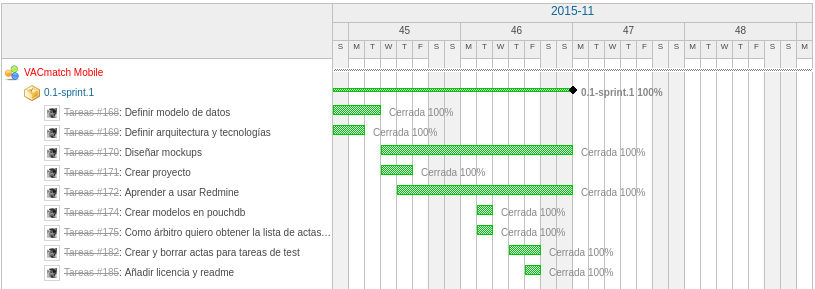
\includegraphics[width=\textwidth]{./img/gant_diagrams/01.png}
          \caption{Diagrama de Gant do sprint 1}
          \label{fig:gant01}
          \end{center}
        \end{figure}

        \begin{figure}[h!]
          \begin{center}
          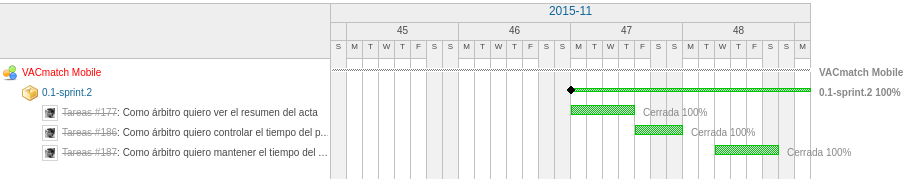
\includegraphics[width=\textwidth]{./img/gant_diagrams/02.png}
          \caption{Diagrama de Gant do sprint 2}
          \label{fig:gant01}
          \end{center}
        \end{figure}

  A planificación inicial de 71 horas de desenvolvemento finalmente cumpliuse 
correctamente, incluso reducindo o tempo empregado ata as 68.

    \subsubsection{Participación na I Lonxa de Financiamento Responsable}
    \label{sec:lonxa}
    Durante este tempo tamén cómpre destacar a participación de VACmatch na I 
Lonxa de Financiamento Responsable en Galicia, permitíndonos presentar o noso 
proxecto ante diversos inversores preocupados pola responsabilidade social das 
empresas.

    \begin{figure}[h!]
          \begin{center}
          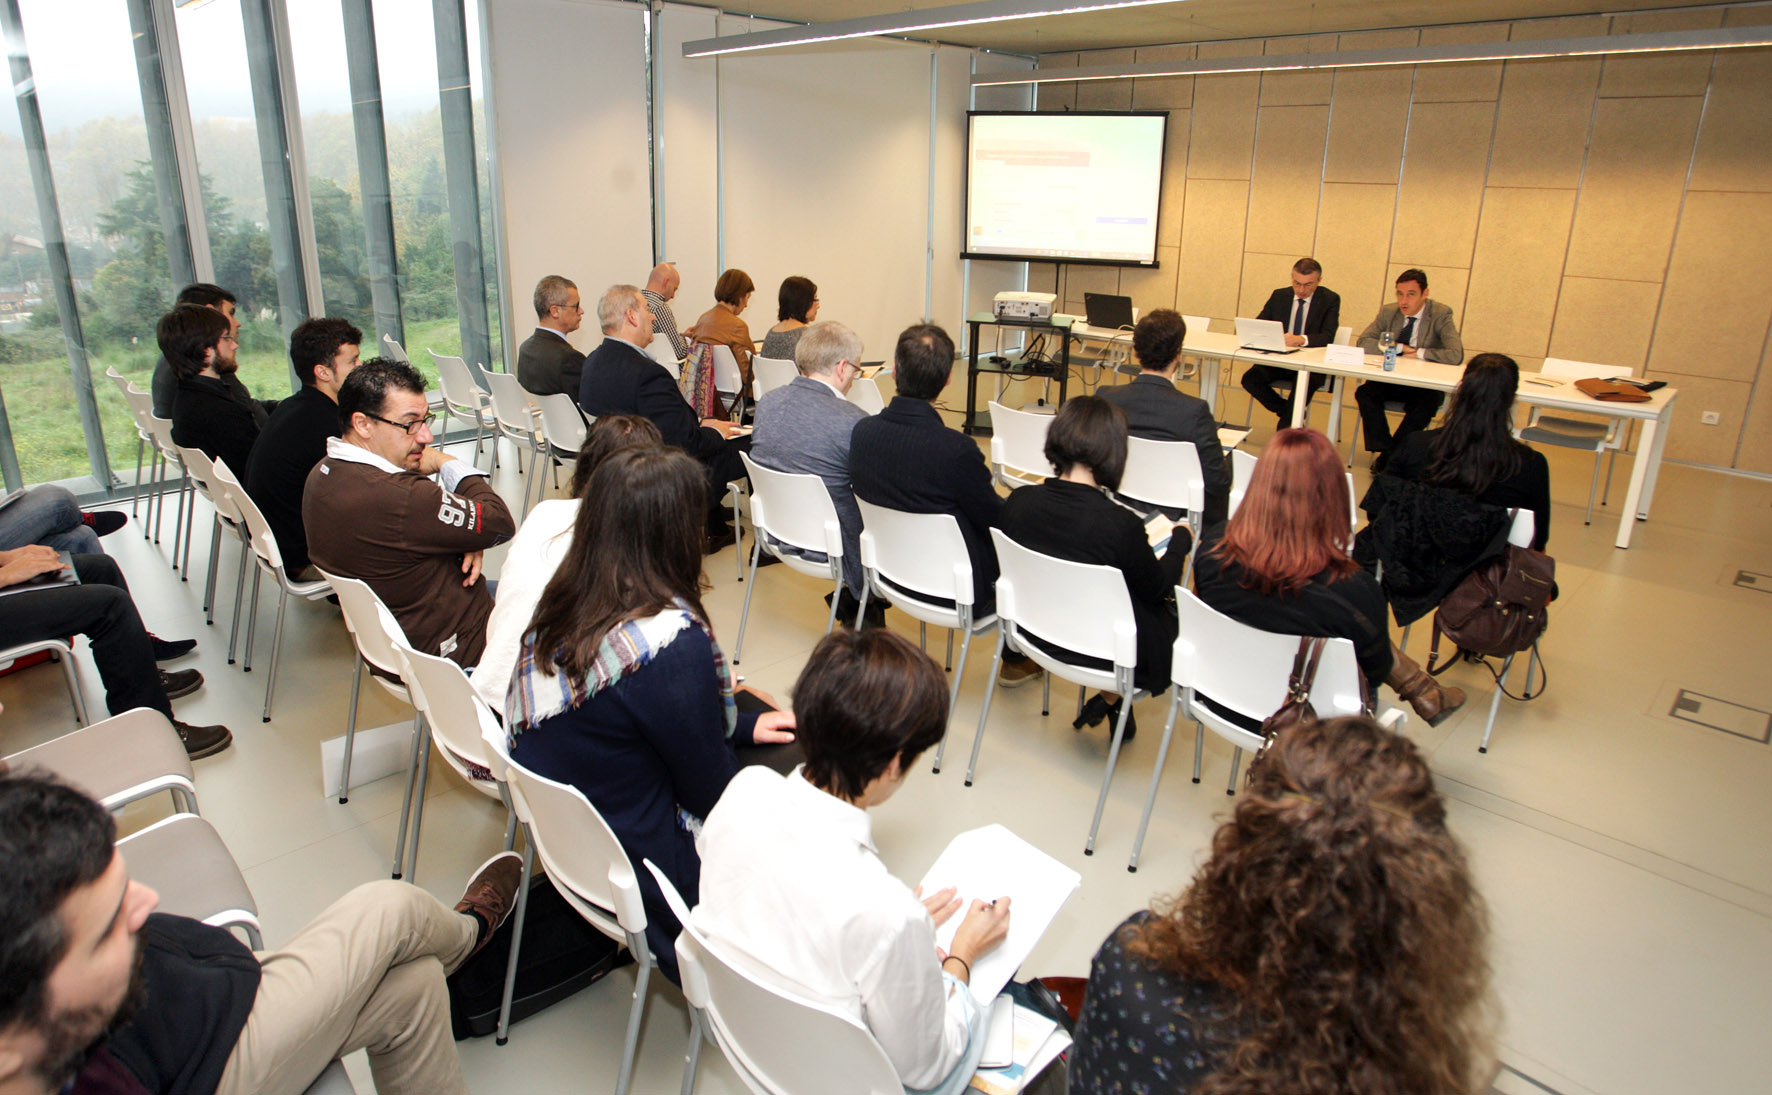
\includegraphics[width=0.8\textwidth]{./img/inversion_responsable.jpg}
          \caption{I Lonxa de Financiamento Responsable}
          \label{fig:lonxa}
          \end{center}
    \end{figure}

        Foi unha experiencia única que nos permitíu introducirnos por primeira 
vez no mundo da inversión en startups e coñecer aos diversos proxectos que se 
presentaron, obtendo tamén feedback dos asistentes e participantes.

    \subsection{3ª iteración. Eventos}

      \subsubsection{Planificación e definición da iteración}
      Esta iteración comeza o 30 de Novembro e remata o 13 de Decembro, unha 
iteración de dúas semanas de duración e céntrase principalmente na xestión de 
eventos dos encontros, tarefas que requiren unha forte planificación e análise 
xa que se busca que ditos eventos sexan o máis xenéricos posibles e facilmente 
adaptables aos diversos deportes.

      Da mesma forma plantéxase crear tipos de eventos que modifiquen tamén a 
propia acta, actualizando na mesma tanto o resultado como as faltas cometidas.

      Por último incorpórase tamén na iteración a posibilidade de convocar e 
editar persoas dun equipo así como algún pequeno erro detectado na última 
iteración.

      \subsubsection{Revisión e feedback}
      Esta iteración centróuse en avanzar a maior velocidade no 
desenvolvemento, pódese observar cómo o número de horas asignadas supera a 
media teórica planificada para o período completo.

      Non se realizou ningunha visita a federacións e centrouse prácticamente 
todo o esforzo, fora do desenvolvemento, en preparar a presentación para a I 
Lonxa de Financiamento Responsable en Galicia da que se falou 
anteriormente na Sección~\ref{sec:lonxa} e na que se obtiveron diversos 
comentarios para enfocar o modelo de negocio e o desenvolvemento da aplicación 
cara o cliente.

      \subsubsection{Tarefas e seguimento}

      A continuación móstranse as diversas tarefas realizadas na iteración:

        \begin{description}
          \item [S3.1] Como árbitro quero poder engadir un evento.
          \item [S3.1.1] Como árbitro quero ver a lista de xogadores para 
asignar un evento.
          \item [S3.1.2] Como árbitro quero poder confirmar engadir un evento.
          \item [S3.1.3] Como árbitro quero engadir unha causa a un evento.
          \item [S3.2] Cómo árbitro quero poder ver a lista de eventos de un 
partido.
          \item [S3.3] Como árbitro quero que se xeneren eventos de comezo e 
fin de partido.
          \item [S3.4] Como árbitro quero que se xeneren eventos ao cambiar de 
parte.
          \item [S3.5] Como árbitro quero que se actualice o resultado ao 
engadir un gol.
          \item [S3.6] Como árbitro quero que se actualicen as faltas 
automáticamente.
          \item [S3.7] Como árbitro quero poder convocar e desconvocar 
xogadores.
          \item [S3.8] Como árbitro quero poder cambiar o dorsal de un xogador 
nun partido determinado.
          \item [S3.9] Como árbitro quero poder borrar un evento.
          \item [S3.10] Como árbitro quero ver a lista de eventos de un partido 
ordenada por tempo e parte.
          \item [S3.11] Mostrar únicamente xogadores convocados ao engadir un 
evento.
          \item [S3.12] Como árbitro quero que ao borrar un evento se 
actualicen os 
resultados e as faltas na Acta.
          \item [S3.12] Erro: Cando non hai ningún evento de cambio de parte 
hai un error.
          \item [S3.13] Erro: Corexir erro cando se engade un evento con causa.
        \end{description}

        \begin{figure}[h!]
          \begin{center}
          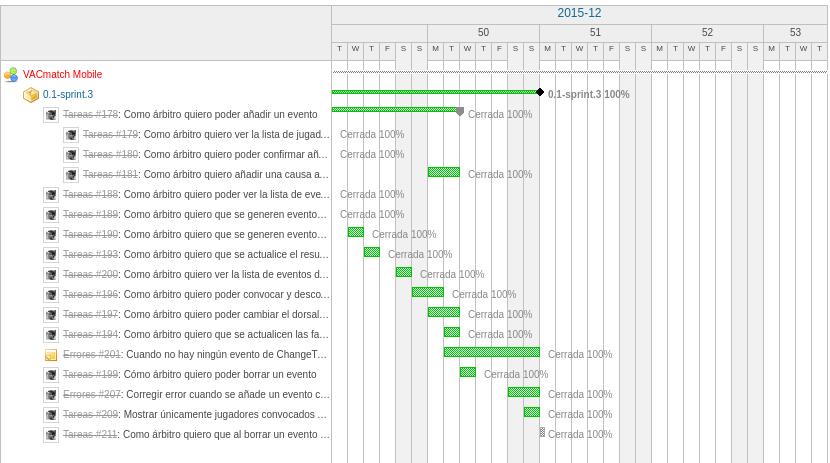
\includegraphics[width=\textwidth]{./img/gant_diagrams/03.png}
          \caption{Diagrama de Gant do sprint 3}
          \label{fig:gant03}
          \end{center}
        \end{figure}

        Finalmente a planificación inicial de 51 horas cumpríuse correctamente 
quedando un extra de 6 horas que foron reasignadas ao outro proxecto.

    \subsection{4ª iteración. Xestión de usuarios e creación offline de actas}

      \subsubsection{Planificación e definición da iteración}
      Esta iteración ten lugar entre o 14 e o 30 de Decembro de 2015 e céntrase 
na autenticación da aplicación que debe integrar unha base de datos remota para 
que os árbitros poidan conectarse co seu usuario e tamén inclúe a creación e 
edición manual de actas que en anteriores iteracións foi engadida únicamente 
para probas internas pero sen realizar as comprobacións necesarias.

      Tamén se planifican tarefas para comezar as primeiras partes da memoria 
do proxecto que incluen a introdución, o estado da arte os fundamentos 
tecnolóxicos.

      \subsubsection{Revisión e feedback}
      Durante este periodo escribíuse unha nova entrada no blog do proxecto 
na que se fixo unha introdución aos fundamentos tecnolóxicos do mesmo, 
explicando a motivación da elección das tecnoloxías e mostrando un exemplo 
moi sinxelo.

      Por último mostrouse tamén a estrutura da aplicación e as partes máis 
importantes do proxecto, pensando en facilitar a introdución no 
desenvolvemento aos posibles interesados en colaborar no mesmo.

      \subsubsection{Tarefas e seguimento}

      O listado de tarefas abordadas durante esta iteración é o seguinte:

        \begin{description}
          \item [S4.1] Como usuario quero poder facer log in.
          \item [S4.2] Engadir diferenciación entre Persoal e Xogadores.
          \item [S4.3] Como usuario quero poder facer log out.
          \item [S4.4] Como árbitro quero poder crear un partido manualmente.
          \item [S4.5] [Memoria] Definir introdución.
          \item [S4.6] [Memoria] Estado da arte.
          \item [S4.7] [Memoria] Fundamentos tecnolóxicos.
          \item [S4.8] [Memoria] Engadir modelo.
          \item [S4.9] Como árbitro quero poder editar un acta creada dende o 
móbil.
          \item [S4.10] Erro: Correxir erro coa variable dialogIsOpen ao editar 
o dorsal de un xogador.
        \end{description}

        \begin{figure}[h!]
          \begin{center}
          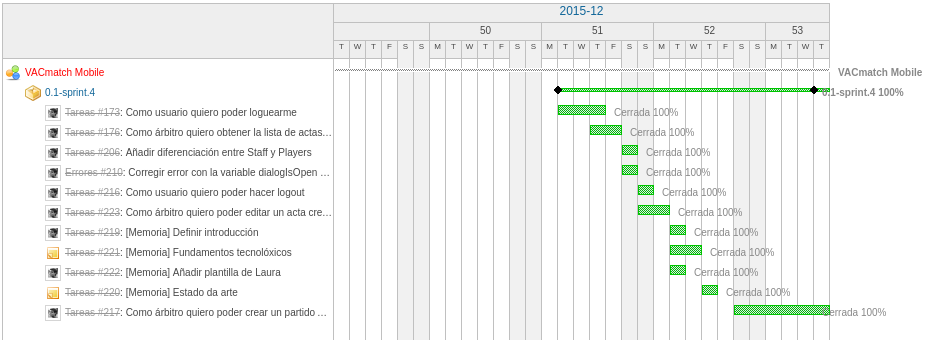
\includegraphics[width=\textwidth]{./img/gant_diagrams/04.png}
          \caption{Diagrama de Gant do sprint 4}
          \label{fig:gant04}
          \end{center}
        \end{figure}

      Esta vez a planificación non foi moi acertada debido a diversos 
imprevistos externos ao proxecto, o que levou a necesidade de mover diversas 
tarefas á seguinte iteración para axustar a planificación incial de 53.5 horas 
as 44 que se realizaron finalmente.

    \subsection{5ª iteración. Sinaturas}

      \subsubsection{Planificación e definición da iteración}
      Esta iteración comeza o día 1 de Xaneiro de 2016 e remata o día 8 
e centrase na última vista da aplicación, aquela que permite xestionar a 
finalización do encontro dando a posibilidade de asinar a acta e engadir 
comentarios por parte do árbitro.

      Na iteración anterior detectáronse varias melloras a incluir como facer 
que por defecto as contas creadas dende a aplicación móbil sexan todas de tipo 
árbitro. Así mesmo facer que se engada a dito usuario como árbitro do encontro 
en tódalas actas que cree esa conta.

      \subsubsection{Revisión e feedback}
      Ao finalizar esta iteración publicóuse unha nova entrada no blog do 
proxecto expoñendo a metodoloxía áxil utilizada para o desenvolvemento así como 
aquelas nas que se basea (Scrum e eXtreme Programming) e a metodoloxía de 
negocio orientada cara o cliente (Lean Startup).

      Por último tamén se publicou o fluxo de traballo que se realiza para 
contribuir ao proxecto co sistema de control de versións Git, co fin de 
facilitar o traballo a futuros contribuidores.

      \subsubsection{Tarefas e seguimento}

      Durante esta iteración realizáronse as seguintes tarefas e das cales se 
pode observar o seu diagrama de Gant na Figura~\ref{fig:gant05}.

        \begin{description}
         \item [S5.1] Como árbitro quero poder asinar un acta.
         \item [S5.2] Como árbitro quero que unha ou varias persoas convocadas 
de cada equipo poidan asinar un acta.
         \item [S5.3] Como árbitro quero poder engadir comentarios a un acta.
         \item [S5.4] Como árbitro quero poder borrar un xogador da lista de 
convocados.
         \item Crear un árbitro ao crear un novo usuario na aplicación móbil.
         \item Engadir o árbitro que ten o usuario asignado nas actas que crea.
        \end{description}

        \begin{figure}[h!]
          \begin{center}
          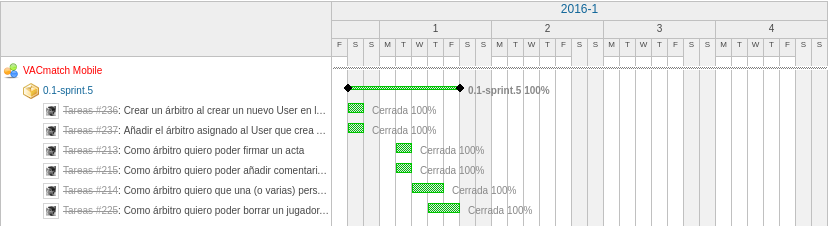
\includegraphics[width=\textwidth]{./img/gant_diagrams/05.png}
          \caption{Diagrama de Gant do sprint 5}
          \label{fig:gant05}
          \end{center}
        \end{figure}

        Nesta iteración a planificación incial de 32 horas foi sobreestimada 
polo sobraron 5 horas de desenvolvemento que foron reasignadas a outro proxecto.

  \section{De empresa a comunidade (Xaneiro 2016 -- Maio 2016)}
  Durante o mes de Xaneiro de 2016 decidíuse abandonar o proxecto de VACmatch 
como iniciativa empresarial por diversos motivos e continuar con él únicamente 
como proxecto comunitario de software libre.

  Motivado por isto, producíuse un parón de aproximadamente un mes de duración 
e ao mesmo tempo comezouse a traballar nunha empresa externa polo que durante 
este período diminuíu considerablemente o tempo dispoñible para continuar co 
proxecto.

  O número de horas total estimado para este período de 6 iteracións é de 189, 
todo nun total de 5 meses, o que supón unha media aproximada de 2 horas 
diarias de desenvolvemento.

    \subsection{6ª e 7ª iteración. Optimización e melloras}
    Motivado pola inestabilidade xerada polos cambios mencionados anteriormente,
non se realizou unha correcta planificación da 6ª iteración e finalmente non 
foi posible realizar ninguha tarefa polo que se decidíu unir ambas iteracións.

      \subsubsection{Planificación e definición da iteración}
      Estas iteracións comezan o 14 de Xaneiro de 2016 e rematan o 29 de 
Febreiro, a pesar de que non se realizou traballo efectivo ata as últimas dúas 
semanas de Febreiro.

      Durante este periodo planificouse unha importante refactorización de 
código co fin de simplificar certas partes do código e facilitar o mantemento 
da aplicación así como revisar a forma na que se crean os identificadores dos 
obxectos en base de datos.

      \subsubsection{Revisión e feedback}
      Como se comentou anteriormente, este foi un sprint marcado por un longo 
parón de aproximadamente un mes e medio durante o que o proxecto non avanzóu 
nin se obtivo ningún tipo de feedback.

      En cambio durante este tempo si se publicaron varias entradas no blog do 
proxecto co fin de poñer ao día de xeito público os últimos avances do proxecto 
e contar diversas decisións técnicas que se adoptaron como a selección da 
licencia para o proxecto, a implementación do sistema de eventos ou a sinatura 
das actas.

      \subsubsection{Tarefas e seguimento}

      Durante esta iteración realizáronse poucas tarefas, todas imputadas ao 
sprint número 7, pero de unha duración considerable como se pode observar no 
diagrama de Gant da Figura~\ref{fig:gant07}.

        \begin{description}
         \item [S7.1] Refactorizar servicios.
         \item [S7.2] Crear clases para cada entidade.
         \item [S7.3] Revisar cómo se crean os identificadores dos obxectos en 
base de datos.
        \end{description}

        \begin{figure}[h!]
          \begin{center}
          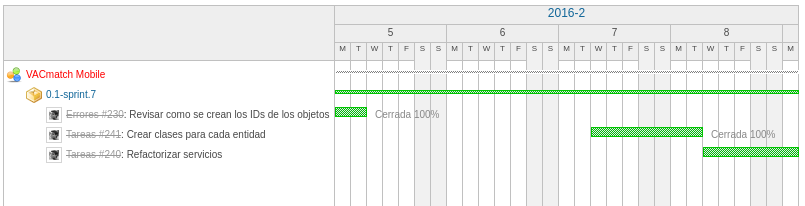
\includegraphics[width=\textwidth]{./img/gant_diagrams/07.png}
          \caption{Diagrama de Gant do sprint 7}
          \label{fig:gant07}
          \end{center}
        \end{figure}

    Para a realización de esta iteración planificóuse un total de 22 horas e 
non se precisou ningunha hora extra para completar o traballo.

    \subsection{8ª iteración. Testing e integración continua}

      \subsubsection{Planificación e definición da iteración}
      A iteración transcorre entre os días 1 e 14 de Marzo.

      Decidíuse engadir tests unitarios para previr futuros erros e facilitar o 
mantemento da aplicación xa que en todo proxecto de certa embergadura, e máis 
en proxectos libres nos que calquera pode colaborar, é importante asegurar que 
os novos cambios que se engadan, non xeneren problemas no funcionamento da 
aplicación.

      Relacionado con este tema tamén se planificou a integración do 
repositorio de código con unha ferramenta de integración continua que facilite 
a execución de este tipo de probas, en este caso Travis CI.

      \subsubsection{Revisión e feedback}
      Durante esta iteración foi preciso publicar unha folla de ruta do 
proxecto no blog do mesmo, requisito fundamental solicitado pola organización 
do Concurso Universitario de Software Libre no que VACmatch se atopa inscrito 
dende o mes de Outubro aproximadamente.

      É por iso que se fixo unha entrada resumo para mostrar as tarefas 
existentes no Redmine do proxecto donde se realiza toda a xestión de 
incidencias así como se resaltou os seguintes pasos a seguir no mesmo como por 
exemplo engadir a internacionalización ou permitir poñer en funcionamento a 
aplicación nun dispositivo móbil.

      \subsubsection{Tarefas e seguimento}

      As seguintes tarefas son as realizadas en esta iteración:

        \begin{description}
         \item [S8.1] Engadir tests aos servizos de Eventos, Persoas, Equipos e 
Actas.
         \item [S8.2] Engadir tests aos servizos de Auth, Árbitros e Sinaturas.
         \item [S8.3] Engadir integración continua con Travis CI.
         \item [S8.4] Engadir campos para confirmar contrasinal e código PIN ao 
crear un usuario.
        \end{description}

        \begin{figure}[h!]
          \begin{center}
          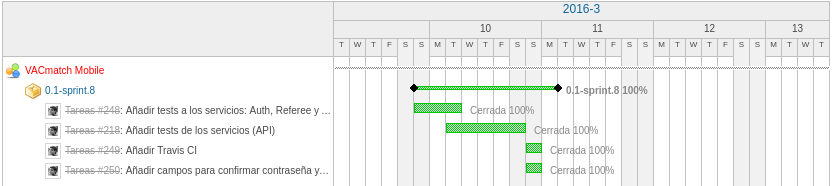
\includegraphics[width=\textwidth]{./img/gant_diagrams/08.png}
          \caption{Diagrama de Gant do sprint 8}
          \label{fig:gant08}
          \end{center}
        \end{figure}

        No diagrama da Figura~\ref{fig:gant08} pódese observar a evolución das 
tarefas ao longo do sprint que inicialmente tivo unha planificación de 37 horas 
pero finalmente alongouse 16 horas extra, obrigando a ampliar a xornada de 
traballo en 2 fines de semana a media xornada co obxectivo de non retrasar a 
execución das tarefas.

    \subsection{9ª e 10ª iteración. Inxección de dependencias}
    Motivado de novo pola inestabilidade no que se dispón para realizar o 
proxecto, finalmente decidíuse integrar de novo estas dúas iteracións en unha.

      \subsubsection{Planificación e definición da iteración}
      Estas iteracións comezan o día 15 de Marzo e rematan o 25 de Abril.

      Detectáronse problemas en Travis xa que non detectaba erros nos tests 
polo que é o primeiro que había que corrixir.

      Tamén se decidíu crear unha barra de notificacións compartida para todos 
os compoñentes da aplicación e engadíronse estados diferentes para as actas co 
fin de mostrar cando un encontro non comezou, cando se está a xogar e cando 
rematou o mesmo.

      Pero a tarefa máis importante xurdíu ao aparecer un problema de 
denpendencias circulares que obrigou a engadir unha factoría para realizar unha 
inxección de dependencias entre os servizos da aplicación xa que varios, 
dependían uns de outros.

      Finalmente planificouse tamén a corrección de diversos erros detectados 
na iteración anterior.

      \subsubsection{Revisión e feedback}
      Durante esta iteración non se publicou ningunha entrada no blog e 
tampouco se recibiron suxerencias.

      \subsubsection{Tarefas e seguimento}

      As tarefas definidas para esta iteración son as seguintes:

      \begin{description}
       \item [S10.1] Engadir textos de error na aplicación.
       \item [S10.2] Crear barra de notificacións para utilizar en calquera 
compoñente.
       \item [S10.3] Erro: Correxir problema de dependencias circulares.
       \item [S10.3.1] Engadir DAOs.
       \item [S10.3.2] Engadir Inxección de Dependencias.
       \item [S10.4] Erro: Mostrar que o partido rematóu na acta.
       \item [S10.4.1] Engadir estados na Acta.
       \item [S10.5] Erro: Como árbitro non debería poder convocar/borrar a un 
xogador que ten eventos asignados.
       \item [S10.6] Erro: Correxir erros varios derivados de engadir inxección 
de dependencias.
       \item [S10.7] Erro: Un evento de comezo de partido non se pode borrar si 
existe algún outro evento creado.
       \item [S10.8] Erro na xestión do estado da Acta.
       \item [S10.9] Erro: Travis CI non funciona correctamente
      \end{description}

        \begin{figure}[h!]
          \begin{center}
          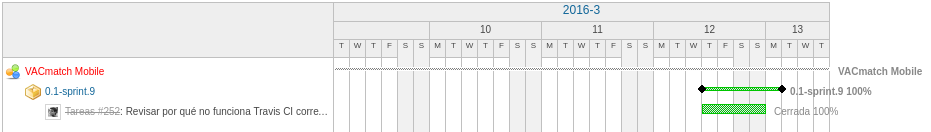
\includegraphics[width=\textwidth]{./img/gant_diagrams/09.png}
          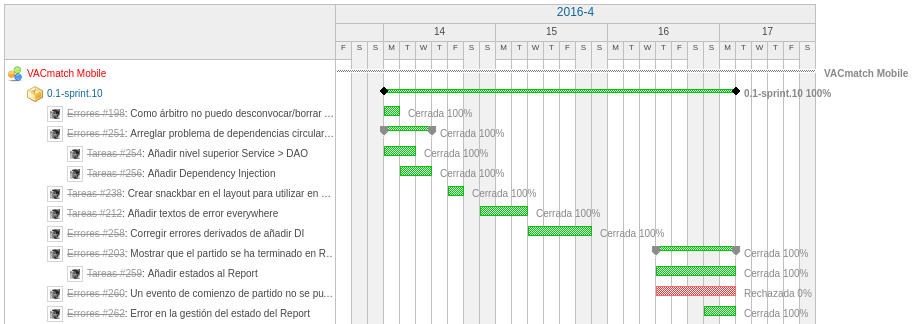
\includegraphics[width=\textwidth]{./img/gant_diagrams/10.png}
          \caption{Diagramas de Gant dos sprints 9 e 10}
          \label{fig:gant10}
          \end{center}
        \end{figure}

    A estimación inicial de horas para esta iteración foi de un total de 78, 
resultando unha vez máis optimista e permitindo que a diferencia de horas coas 
reais, 66, poidesen ser reasignadas ao proxecto de VACmatch Web.

    \subsection{Release 0.2.0: Usabilidade en menús}

      \subsubsection{Planificación temporal}
      Esta iteración transcorre entre o día 25 de Abril e o 9 de Maio.

      \subsubsection{Definición da iteración}
      Unha iteración con unha sola tarefa pero de un tamaño suficiente para 
cubrir a totalidade do sprint, centrada en engadir os enlaces que faltaban no 
menú lateral esquerdo e no superior dereito, certos botóns de retroceso e 
corexidos diversos erros menores.

      \subsubsection{Concurso Universitario de Software Libre}
      Así mesmo, durante este iteración recibíuse o ``Premio al mejor proyecto 
de tecnologías móviles`` do Concurso Universitario de Software Libre (CUSL), un 
concurso onde participaron máis de 75 estudantes de toda España e donde se 
expuxeron 47 proxectos de código libre.

      Fomos invitados a participar na fase final que tivo lugar os días 5 e 6 
de Maio na Universidade de Sevilla na que presentar o proxecto ante 
representantes de diversas empresas de software libre españolas que tamén 
participaron con diversas charlas sobre os seus modelos de negocio e as 
vantaxes do software libre a nivel empresarial.

      Foi unha gran experiencia a compartida con todos os finalistas e 
asistentes e, por suposto, os custes da viaxe foron subvencionados pola 
organización e o premio finalmente foi de 500 \euro{} en metálico.

    \begin{figure}[h!]
          \begin{center}
            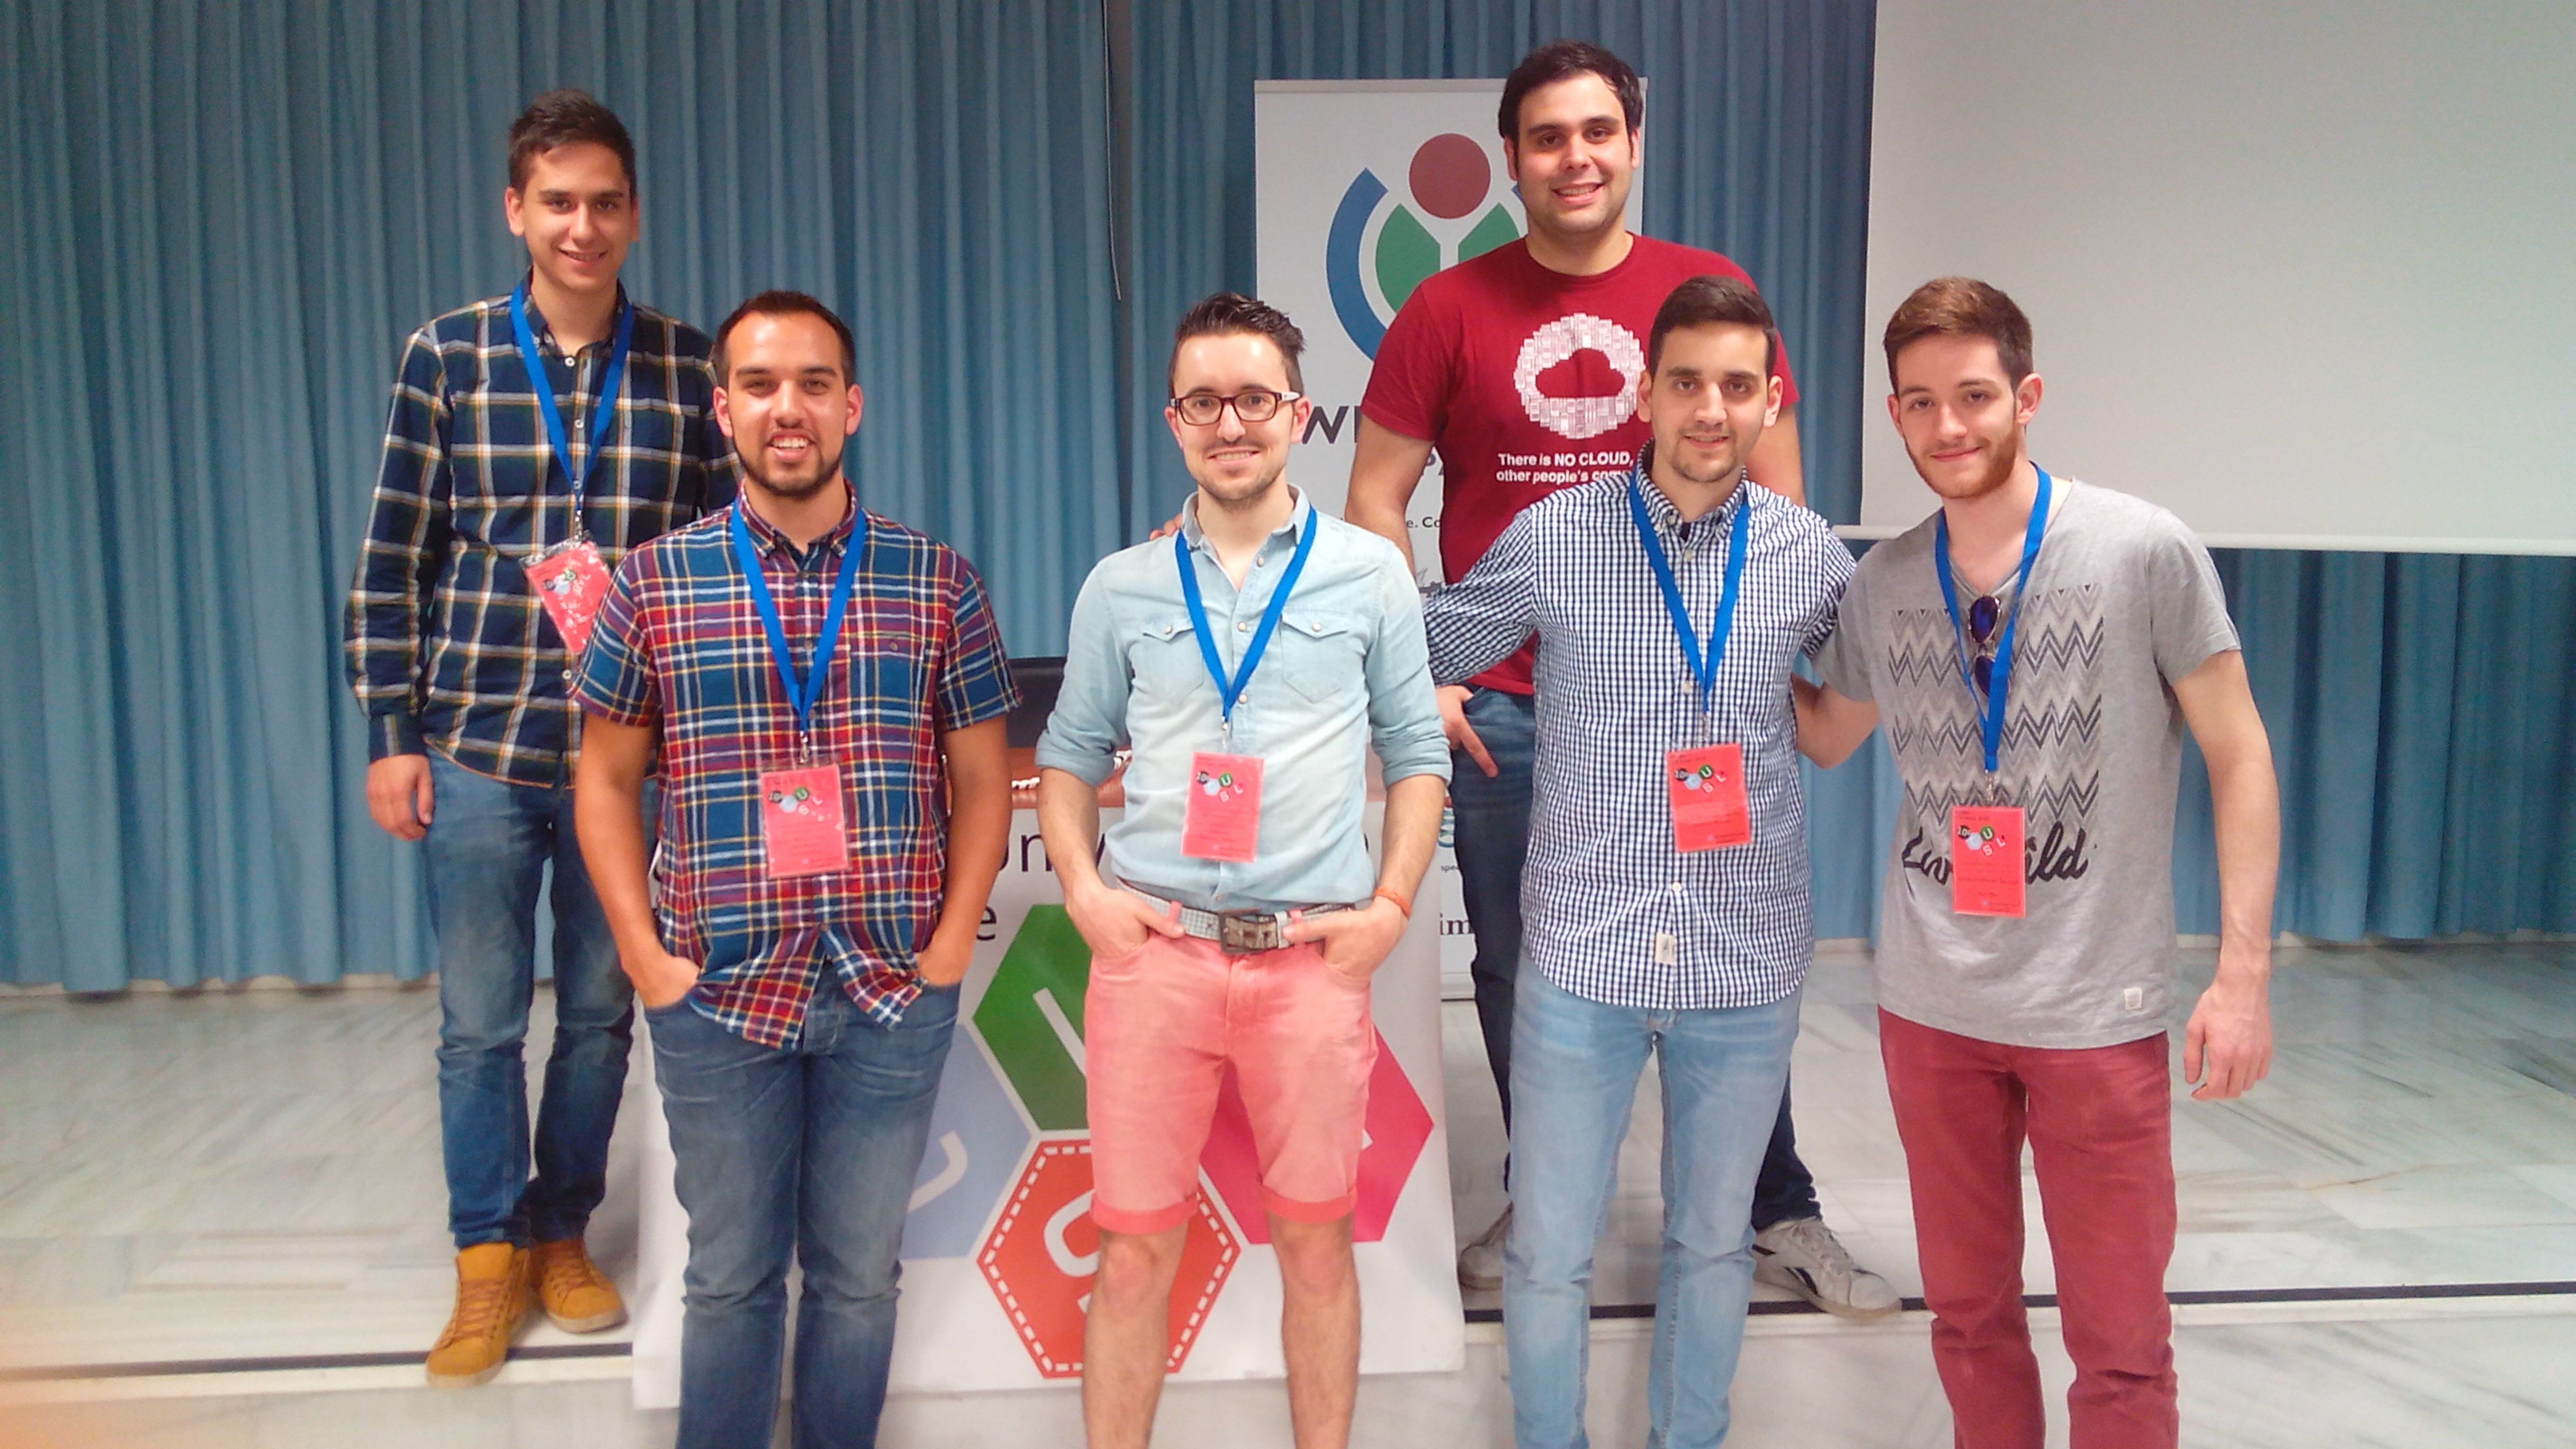
\includegraphics[width=0.8\textwidth]{./img/final_cusl.jpg}
            \caption{Finalistas CUSL}
          \end{center}
    \end{figure}

      \subsubsection{Revisión e feedback}

      \subsubsection{Tarefas e seguimento}
        \begin{itemize}
        \item Revisar os links nos menús e engadir información.
        \end{itemize}


    \subsection{Release 0.2.1: I18n e app híbrida}

      \subsubsection{Planificación temporal}
      Esta iteración comeza o día 9 e remata o 24 Maio.

      \subsubsection{Definición da iteración}
      A tarefa de maior tamaño que se planificou en esta iteración foi a 
internacionalización coa librería React Intl xa que supón modificar todas as 
vistas da aplicación.

      Posteriormente engadíuse Apache Cordova para permitir crear aplicacións 
híbridas que funcionen en diversos sistemas operativos móbiles e por suposto, 
tamén se incluíu no repositorio de código, a documentación sobre cómo arrancar 
unha base de datos CouchDB para utilizar como backend e sobre cómo realizar a 
compilación da aplicación para executar nun sistema operativo móbil.

      \subsubsection{Revisión e feedback}

      \subsubsection{Tarefas e seguimento}
        \begin{itemize}
        \item Engadir internacionalización.
        \item Crear app híbrida con Apache Córdova.
        \end{itemize}
%
% ----------- WORK IN PROGRESS
%
    \subsection{Release 0.2.2: Imáxe corporativa e revisión de erros}
    Imaxe corporativa VACmatch, bugfix
    Memoria a saco
      \subsubsection{Planificación temporal}
      \subsubsection{Definición da iteración}
      \subsubsection{Revisión e feedback}
      \subsubsection{Tarefas e seguimento}
% 
%     \subsection{Release 0.3.0: Usabilidade móbil e entrega continua}
%     Por cordova: dialogos -> ventás, transición carga, migrar taiga.io, Travis + 
% Docker
%       \subsubsection{Planificación temporal}
%       \subsubsection{Definición da iteración}
%       \subsubsection{Revisión e feedback}
%       \subsubsection{Tarefas e seguimento}


%%% Local Variables:
%%% mode: latex
%%% TeX-master: "../root"
%%% End:
